\documentclass[professionalfonts, xcolor=table]{beamer}
%% \documentclass[professionalfonts, xcolor=table, handout]{beamer}
%% \usepackage{pgfpages}
%% \pgfpagesuselayout{4 on 1}[a4paper,border shrink=5mm, landscape]
\usepackage{fontspec}
\usepackage{amsmath,amssymb}
\usepackage{tikz}
\usetikzlibrary{positioning, matrix, arrows.meta, shapes.geometric, calc,
  decorations.pathmorphing, decorations.pathreplacing, fit, shapes.multipart}
\usepackage{mathabx}
\usepackage{mathtools}
\usepackage{mathpartir}
\usepackage{fancyvrb}
\usepackage{stmaryrd}
\usepackage[absolute,overlay]{textpos}

\defaultfontfeatures{Mapping=tex-text,Scale=MatchLowercase}
% \setmainfont{Libertinus Serif}
% \setsansfont{Libertinus Sans}
\setmonofont{Menlo Regular}
\usetheme{CambridgeUS}

\definecolor{lightg}{RGB}{217,232,225}
\definecolor{darkg}{RGB}{6,81,42}

\useinnertheme{circles}
\setbeamertemplate{enumerate item}[default]
\usecolortheme{spruce}
\usefonttheme{serif}
\setbeamerfont*{frametitle}{series=\bfseries}
\setbeamercolor{alerted text}{fg=red}
\setbeamertemplate{navigation symbols}{}
\setbeamercolor{emphC}{fg=red}
\setbeamercolor{block title}{bg = darkg, fg=white!80}
\setbeamercolor{block body}{bg = lightg, fg=black}
\setbeamercolor{itemize item}{fg=darkg}
\setbeamercolor{description item}{fg=darkg}

\newcommand{\scon}{\mathbin{\varstar}}
\newcommand{\ocon}{%
  \mathbin{\mbox{$\mathrlap{\cup}\hspace*{.15em}
      \raisebox{.01em}[0ex][0ex]{$\scon$}$\hspace*{.07em}}}}
\newcommand{\medocon}{
  \raisebox{-0.3ex}{\resizebox{0.63em}{!}{$\scon$}} \hspace{-2.4ex} \bigcup}
\newcommand{\wand}{%
 \mathrel{\mbox{$\hspace*{-0.03em}\mathord{-}\hspace*{-0.66em}
  \mathord{-}\hspace*{-0.36em}\mathord{\scon}$\hspace*{-0.005em}}}}
\newcommand{\defeq}{\mathbin{\overset{\mathrm{def}}{=}}}
\newcommand{\emphd}[1]{{\bfseries #1}}
\newcommand{\emphr}[2]{\alert<#1>{#2}}
\newcommand{\bracket}[1]{[#1]}
\makeatletter\let\frametextheight\beamer@frametextheight\makeatother
\newcommand\credit[1]{%
  \begin{textblock*}{\paperwidth}(0pt,\textheight)
    \raggedleft #1\hspace{.5em}
\end{textblock*}}
\newcommand{\pguards}[1]{\llbracket #1 \rrbracket}

\title[Mechanized Verification]{Mechanized Verification of \\
  Graph-manipulating Programs}
\author[Wang, Cao, Mohan, Hobor]{\hspace{-0.5em}\underline{Shengyi Wang}$^{\dagger}$,
  Qingxiang Cao$^{\ddagger}$, Anshuman Mohan$^{\dagger}$, Aquinas Hobor$^{\dagger}$
  \hspace*{-0.5em}}
\institute[NUS]{$
\includegraphics[height=0.12\textwidth]{NUS_logo_full-horizontal.jpg}
  ~\raisebox{2em}{$(\dagger)$}$
  $\qquad \qquad \qquad$ $
\includegraphics[height=0.12\textwidth]{sjtubannerblue.png}~
  ~\raisebox{2em}{$(\ddagger)$}$ \hspace*{-1.25em}}
\date[OOPSLA 2019]{Object-Oriented Programming, Systems, Languages \& Applications \\
  October 24, 2019}

\begin{document}
\begin{frame}
  \titlepage
\end{frame}

\section{Introduction}

\begin{frame}{Our Focus}
We would like to verify \alert{graph-manipulating} programs written in \alert{real C}
with end-to-end \alert{machine-checked} correctness proofs.
\begin{itemize}
\item Hard to reason about
\item Occur in critical areas
\item C is hard
\item Machine-checked proofs are hard
\end{itemize}
\end{frame}

\begin{frame}{Our Strategy}
Use \alert{CompCert} and \alert{Verified Software Toolchain} (VST) to certify  code against strong specifications expressed with \alert{mathematical graphs}.
\begin{itemize}
\item CompCert + VST = 50+ person-years
\item No changes to CompCert
\item Add 1\% to VST
\item Vanilla separation logic (using $\wand$ and quantifiers).
\item This framework is \alert{powerful enough to verify real code}.
\end{itemize}
\end{frame}

\begin{frame}{Our Workflow}
  
\begin{tikzpicture}[remember picture,overlay, on grid,
      ourlib/.style={rounded corners=4pt, line width=0.8pt},
      cmd/.style={rectangle, fill=yellow!50!white, draw=black, rounded corners=4pt},
      file/.style={rounded corners=2pt, line width=1pt, fill=yellow!50!white},
      ->/.style={-Stealth, line width=1pt}]
    \path
    coordinate (nw) at ($(current page.north west) + (0.25, -1.5)$)
    coordinate (ne) at ($(current page.north east) + (-0.25, -1.5)$)
    coordinate (sw) at ($(current page.south west) + (0.25, 0.5)$)
    coordinate (se) at ($(current page.south east) + (-0.25, 0.5)$)
    coordinate (cright) at ($(current page.south west) + (2.85, 0.5)$)
    coordinate (asmleft) at ($(current page.south east) + (-2.85, 0.5)$)
    coordinate (coqleft) at ($(current page.south west)!.5!(current page.south east) +
    (-0.5, 0.5)$)
    coordinate (coqright) at ($(current page.south west)!.5!(current page.south east) +
    (0.5, 0.5)$);
    \draw [ourlib, fill=green!20!white] (nw) rectangle ($(sw) + (0.8, 0)$);
    \node at ($(nw)!.5!(sw) + (0.4, 0)$)
          {\rotatebox{-90}{\textsf{Mathematical Graph Library}}};
    \draw [ourlib, fill=red!20!white] (ne) rectangle ($(se) + (-0.8, 0)$);
    \node at ($(ne)!.5!(se) + (-0.4, 0)$)
          {\rotatebox{-90}{\textsf{Verified Software Toolchain (VST)}}};
    \draw [ourlib, fill=green!20!white] ($(nw) + (1.6, 0)$) rectangle
    ($(ne) + (-1.6, -0.8)$);
    \node at ($(nw)!.5!(ne) + (0, -0.4)$) {\textsf{Spatial Graph Library}};

    \draw [ourlib, fill=green!20!white] ($(nw) + (1.6, -1.6)$) -- ++(0, -0.8) --
    ++(1.6, 0) -- ++(0, -0.8) -- ++(-1.6, 0) -- ++(0, -0.8) -- ++(3.6, 0) --
    ++(0, 0.8) -- ++(-1.6, 0) -- ++(0, 0.8) -- ++(2, 0) -- ++(0, -0.5) -- ++(-1.6, 0)
    -- ++(0, -1.4) -- ++(3.6, 0) -- ++(0, 1.4) -- ++(-1.6, 0) -- ++(0, 0.5) -- ++(2, 0)
    -- ++(0, -0.8) -- ++(-1.6, 0) -- ++(0, -0.8) -- ++(3.6, 0) -- ++(0, 0.8) --
    ++(-1.6, 0) -- ++(0, 0.8) -- ($(ne) + (-1.6, -2.4)$) -- ++(0, 0.8) -- cycle;
    \node at ($(nw)!.5!(ne) + (0, -2)$)
          {\textsf{Verification of a Graph-Manipulating Function}};
    \draw [ourlib, fill=red!20!white] ($(sw) + (1.6, 0)$) -- ++(0, 0.8) --
    ($(cright) + (0.6, 0.8)$) -- ++(0, 1.8) -- ($(coqleft) + (-0.6, 2.6)$) --
    ++(0, -1.8) -- ($(coqright) + (0.6, 0.8)$) -- ++(0, 1.8) --
    ($(asmleft) + (-0.6, 2.6)$) -- ++(0, -1.8) -- ($(se) + (-1.6, 0.8)$) --
    ++(0, -0.8) -- cycle;
    \node at ($(sw)!.5!(se) + (0, 0.4)$) {\textsf{The CompCert Project}};
    \node (P0) at ($(nw) + (2.2, -3.6)$) {$\{P_0\}$};
    \node (C1) [cmd, right=1.2 of P0] {$C_1$};
    \node (P1) [right=2.4 of P0] {$\{P_1\}$};
    \node (P2) [right=2.4 of P1] {$\{P_2\}$};
    \node (P3) [right=2.4 of P2] {$\{P_3\}$};
    \node (C2) [cmd, right=2.4 of C1] {$C_2$};
    \node (C3) [cmd, right=2.4 of C2] {$C_3$};
    \node (etc) [right=0.9 of P3] {\bf\ldots};
    \draw [file] ($(sw)!.5!(se) + (-0.5, 1.2)$) -- ++(1, 0) -- ++ (0, 1.1) --
    +(-0.3, 0.3) -- +(-1, 0.3) -- cycle ++(1, 1.1) -- ++(-0.3, 0) -- ++(0, 0.3);
    \node at ($(sw)!.5!(se) + (0, 1.9)$) {\textsf{Coq}};
    \draw [file] ($(sw) + (1.6, 1.2)$) -- ++(1, 0) -- ++ (0, 1.1) --
    +(-0.3, 0.3) -- +(-1, 0.3) -- cycle ++(1, 1.1) -- ++(-0.3, 0) -- ++(0, 0.3);
    \node at ($(sw) + (2.1, 1.9)$) {\textsf{C}};
    \draw [file] ($(se) + (-2.6, 1.2)$) -- ++(1, 0) -- ++ (0, 1.1) --
    +(-0.3, 0.3) -- +(-1, 0.3) -- cycle ++(1, 1.1) -- ++(-0.3, 0) -- ++(0, 0.3);
    \node at ($(se) + (-2.1, 1.9)$) {\textsf{Asm}};
    \draw [->, dashed] ($(sw)!.5!(se) + (-0.3, 2.6)$) .. controls ++(-0.3, 0.5) and
    ($(C1.south) + (0.3, -1)$) .. (C1.south);
    \draw [->, dashed] ($(sw)!.5!(se) + (-0.2, 2.6)$) -- (C2.south);
    \draw [->, dashed] ($(sw)!.5!(se) + (-0.1, 2.6)$) .. controls ++(0.3, 0.5) and
    ($(C3.south) + (-0.3, -1)$) .. (C3.south);
    \draw [->, dashed] ($(sw)!.5!(se) + (0, 2.6)$) .. controls ++(0.4, 0.4) and
    ($(etc.south) + (-0.3, -1.2)$) .. (etc.south);
    \node at ($(cright)!.5!(coqleft) + (0, 1.9)$) {\begin{tabular}{c} \textsf{Parser,}
        \\ \textsf{Simplifier} \end{tabular}};
    \node at ($(coqright)!.5!(asmleft) + (0, 1.9)$) {\begin{tabular}{c}
        \textsf{Verified} \\ \textsf{Compiler} \end{tabular}};
    \draw [->] ($(cright) + (0, 1.9)$) -- ++(0.6, 0);
    \draw [->] ($(coqleft) + (-0.6, 1.9)$) -- ++(0.6, 0);
    \draw [->] ($(coqright) + (0, 1.9)$) -- ++(0.6, 0);
    \draw [->] ($(asmleft) + (-0.6, 1.9)$) -- ++(0.6, 0);

    %% left interface
    \draw [line width=2pt] ($(nw) + (1.8, -0.4)$) -- +(-0.4, 0) +(-0.7, 0) --
    +(-1.2, 0) +(-0.6, -0.2) arc [start angle=-90, end angle=90, radius=0.2];
    \fill ($(nw) + (1.2, -0.4)$) circle [radius=0.1];
    \draw [line width=2pt] ($(nw) + (1.8, -2)$) -- +(-0.4, 0) +(-0.7, 0) --
    +(-1.2, 0) +(-0.6, -0.2) arc [start angle=-90, end angle=90, radius=0.2];
    \fill ($(nw) + (1.2, -2)$) circle [radius=0.1];
    \draw [line width=2pt] ($(se) + (-0.6, 0.4)$) -- +(-0.4, 0) +(-0.7, 0) --
    +(-1.2, 0) +(-0.6, -0.2) arc [start angle=-90, end angle=90, radius=0.2];
    \fill ($(se) + (-1.2, 0.4)$) circle [radius=0.1];

    %% right interface
    \draw [line width=2pt] ($(ne) + (-1.8, -0.4)$) -- +(0.4, 0) +(0.7, 0) --
    +(1.2, 0) +(0.6, 0.2) arc [start angle=90, end angle=270, radius=0.2];
    \fill ($(ne) + (-1.2, -0.4)$) circle [radius=0.1];
    \draw [line width=2pt] ($(ne) + (-1.8, -2)$) -- +(0.4, 0) +(0.7, 0) --
    +(1.2, 0) +(0.6, 0.2) arc [start angle=90, end angle=270, radius=0.2];
    \fill ($(ne) + (-1.2, -2)$) circle [radius=0.1];

    %% up interface
    \draw [line width=2pt] ($(ne)!.5!(nw) + (0, -1.8)$) -- +(0, 0.4) +(0, 0.7) --
    +(0, 1.2) +(0.2, 0.6) arc [start angle=0, end angle=-180, radius=0.2];
    \fill ($(ne)!.5!(nw) + (0, -1.2)$) circle [radius=0.1];
    \draw [line width=2pt] ($(ne)!.5!(nw) + (2, -1.8)$) -- +(0, 0.4) +(0, 0.7) --
    +(0, 1.2) +(0.2, 0.6) arc [start angle=0, end angle=-180, radius=0.2];
    \fill ($(ne)!.5!(nw) + (2, -1.2)$) circle [radius=0.1];
    \draw [line width=2pt] ($(ne)!.5!(nw) + (-2, -1.8)$) -- +(0, 0.4) +(0, 0.7) --
    +(0, 1.2) +(0.2, 0.6) arc [start angle=0, end angle=-180, radius=0.2];
    \fill ($(ne)!.5!(nw) + (-2, -1.2)$) circle [radius=0.1];
  \end{tikzpicture}
\end{frame}

\begin{frame}{Our Results}
We have verified half a dozen graph algorithms, including:
\begin{itemize}
\item Graph visiting/coloring; ditto for DAG
\item Graph reclamation (\emph{i.e.} spanning tree followed by tree reclamation)
\item Graph copy
\item Union-find (both for heap- and array-represented nodes)
\item Garbage collector for CertiCoq project
  \pause
\begin{itemize}
\item Generational OCaml-style GC for a purely functional language
\item $\approx$400 lines of (rather devilish) C
\item We find two places where C is too weak to define an OCaml-style GC
\end{itemize}
\end{itemize}
\end{frame}

\begin{frame}{Statistics}
\small
  \centering
  \rowcolors{1}{lightg}{white}
  \scalebox{1.2}{
  \begin{tabular}{|l|c|r|}\hline
    \bf{Component} & \bf{Files} & \bf{LOC} \\\hline
    Common Utilities & 10 & 2,842 \\
    Math Graph Library & 19 & 12,723\\
    Memory Model \& Logic & 13 & 2,373 \\
    Spatial Graph Library  & 10 & 6,458 \\
    Integration into VST  & 12 & 1,917 \\\hline
    Examples (excluding GC) & 13 & 3,290 \\\hline
    GC, subdivided into & 18 & 14,170 \\
%    $\bullet$ GC graphs (Math \& Spatial) & 2 & 7,382 \\
    $\bullet$ mathematical graph & 1 & 5,764 \\
    $\bullet$ spatial graph & 1 & 1,618 \\
    $\bullet$ function specifications & 1 & 461 \\
    $\bullet$ function Hoare proofs & 14 & 3,062 \\
    $\bullet$ isomorphism proof & 1 & 3,265 \\ \hline
    \bf{Total Development} & 95 & 43,773 \\\hline
  \end{tabular}}
\end{frame}

\section{Motivation}

\begin{frame}{Union-Find Algorithm: Problem}
  \centering
  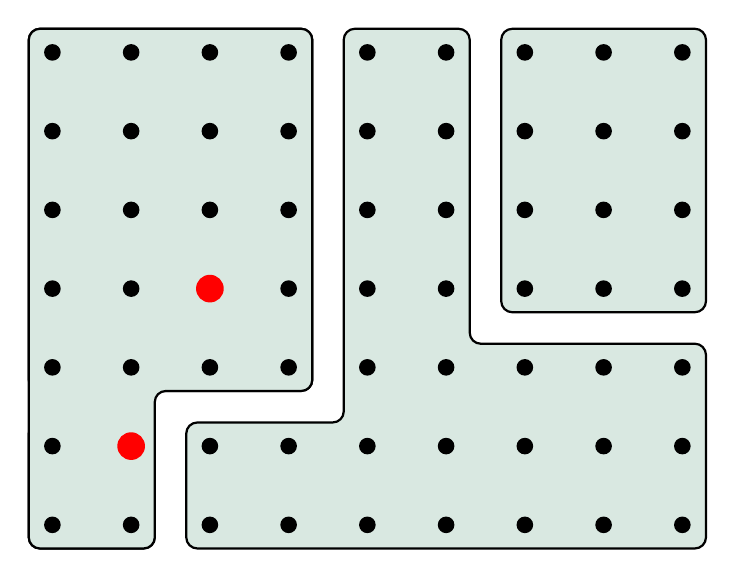
\begin{tikzpicture}[rounded corners]
    \uncover<2,3>{\draw[thick, fill=lightg] (-0.3, -0.3) rectangle (1.3, 1.3);}
    \uncover<2,3>{\draw[thick, fill=lightg] (-0.3, 1.7) rectangle (3.3, 6.3);}
    \uncover<2->{\draw[thick, fill=lightg] (5.7, 2.7) rectangle (8.3, 6.3);}
    \uncover<2->{\draw[thick, fill=lightg] (1.7, -0.3) -- (8.3, -0.3) -- (8.3, 2.3) --
      (5.3, 2.3) -- (5.3, 6.3) -- (3.7, 6.3) -- (3.7, 1.3) -- (1.7, 1.3) -- cycle;}
    \draw<4->[thick, fill=lightg] (-0.3, -0.3) -- (1.3, -0.3) -- (1.3, 1.7) --
    (3.3, 1.7) -- (3.3, 6.3) -- (-0.3, 6.3) -- cycle;
    \foreach \x in {0, ..., 8}
    \foreach \y in {0, ..., 6}
    \fill[black] (\x, \y) circle (3pt);
    \fill<3->[red] (1, 1) circle (5pt);
    \fill<3->[red] (2, 3) circle (5pt);
  \end{tikzpicture}
\end{frame}

\begin{frame}[fragile]{Union-Find Algorithm: Find}
  \begin{columns}[c]
    \column{.6\textwidth}
    \centering
   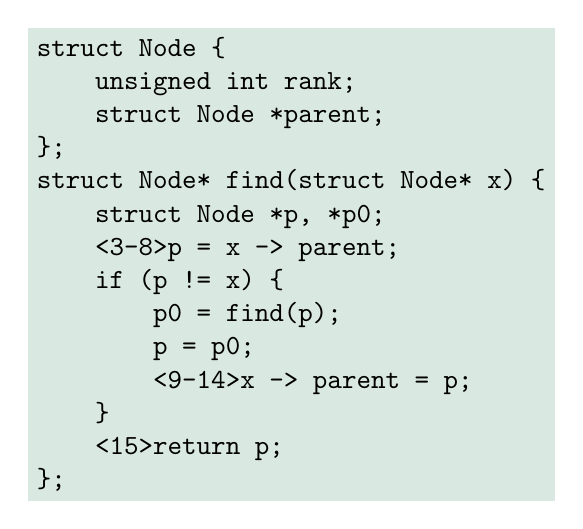
\begin{tikzpicture}
      \node [rectangle, fill=lightg] {
\begin{BVerbatim}[commandchars=\\\[\]]
\emphd[struct] Node {
    unsigned int rank;
    \emphd[struct] Node *parent;
};
\emphd[struct] Node* find(\emphd[struct] Node* x) {
    \emphd[struct] Node *p, *p0;
    \emphr[3-8][p = x -> parent;]
    \emphd[if] (p != x) {
        p0 = find(p);
        p = p0;
        \emphr[9-14][x -> parent = p;]
    }
    \emphr[15][\emphd[return] p;]
};
\end{BVerbatim}
      };
   \end{tikzpicture}
   \column{.4\textwidth}
   \centering
   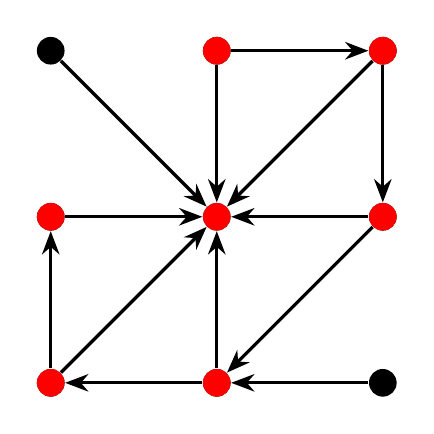
\begin{tikzpicture}[
       gn/.style={circle, inner sep=0pt, minimum size=10pt, fill=black},
       rn/.style={circle, inner sep=0pt, minimum size=10pt, fill=darkg},
       mn/.style={circle, inner sep=0pt, minimum size=10pt, fill=red},
       ->/.style={-Stealth, very thick}]
     \matrix[row sep=50, column sep=50]{
       \node[gn] (g1) {}; & \node<1,3-13,15->[gn] (g2) {};
       \node<2,14>[mn] (g2) {}; & \node<1-2,4-12,14->[gn] (g3) {};
       \node<3,13>[mn] (g3) {}; \\
       \node<1-6,8,10->[gn] (g4) {}; \node<7,9>[mn] (g4) {}; &
       \node<1-7,9-14>[rn] (g5) {}; \node<8,15>[mn] (g5) {}; &
       \node<1-3,5-11,13->[gn] (g6) {}; \node<4, 12>[mn] (g6) {}; \\
       \node<1-5,7-9,11->[gn] (g7) {}; \node<6,10>[mn] (g7) {}; &
       \node<1-4,6-10,12->[gn] (g8) {}; \node<5,11>[mn] (g8) {}; &
       \node[gn] (g9) {}; \\
     };
     \draw [->] (g1) to (g5);
     \draw<1-13> [->] (g2) to (g3);
     \draw<14-> [->] (g2) to (g5);
     \draw<1-12> [->] (g3) to (g6);
     \draw<13-> [->] (g3) to (g5);
     \draw<1-11> [->] (g6) to (g8);
     \draw<12-> [->] (g6) to (g5);
     \draw [->] (g9) to (g8);
     \draw<1-10> [->] (g8) to (g7);
     \draw<11-> [->] (g8) to (g5);
     \draw<1-9> [->] (g7) to (g4);
     \draw<10-> [->] (g7) to (g5);
     \draw [->] (g4) to (g5);
   \end{tikzpicture}
  \end{columns}
\end{frame}

\begin{frame}{Union-Find Algorithm: The Specification of Find}
  \centering
  \colorbox{lightg}{\parbox{.9\textwidth}{
      \begin{description}
      \item[{\bf PRE:}] $\mathtt{graph\_rep}(\gamma) \wedge \mathtt{vvalid}(\gamma, x)$
      \item[{\bf POST:}] $\exists \gamma', \mathit{ret}\;\text{.}\;\mathtt{graph\_rep}(\gamma')\wedge\mathtt{uf\_eq}(\gamma, \gamma') \wedge \mathtt{root}(\gamma', x, \mathit{ret})$
  \end{description}}}
  \pause
  \vskip10pt
  \colorbox{lightg}{\parbox{.9\textwidth}{
      \begin{itemize}[<+->]
      \item How to define $\gamma$, the mathematical graph?
      \item How to define $\mathtt{graph\_rep}(\gamma)$, the spatial
        representation of the graph in memory ?
      \item How to define other predicates, such as
        $\mathtt{uf\_eq}(\gamma, \gamma')$, the graph equivalence and
        $\mathtt{root}(\gamma', x, \mathit{ret})$, the root of $x$ in $\gamma'$
        is $\mathit{ret}$?
      \end{itemize}
    }}
\end{frame}

\section{The Mathematical Graph Library}
\subsection{Core Definitions}

\begin{frame}{Graph Library: Definition of Graph and Path}
\small
    \begin{columns}[c]
      \column{.4\textwidth}
      \centering
      \colorbox{lightg}{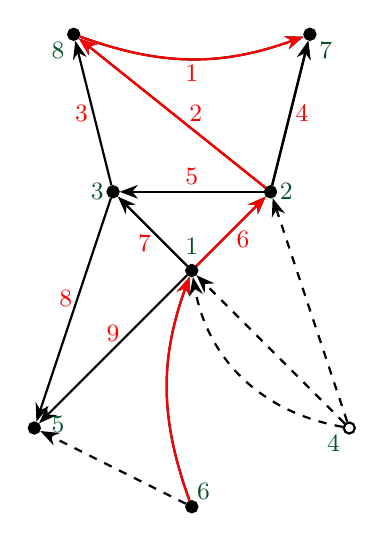
\begin{tikzpicture}
          [vad/.style={circle, fill=black, draw=black, thick,
              inner sep=0pt, minimum size=4pt},
            inv/.style={circle, draw=black, thick, inner sep=0pt, minimum size=4pt},
            ->/.style={thick, arrows={-Stealth}}]
          \node[vad] (n1) at (0, 0) {};
          \node[vad] (n2) at (1, 1) {};
          \node[vad] (n3) at (-1, 1) {};
          \node[inv] (n4) at (2, -2) {};
          \node[vad] (n5) at (-2, -2) {};
          \node[vad] (n6) at (0, -3) {};
          \node[vad] (n7) at (1.5, 3) {};
          \node[vad] (n8) at (-1.5, 3) {};
          \draw<1-4>[->] (n1) to (n2);
          \draw<5->[->, red] (n1) to (n2);
          \draw[->] (n1) to (n3);
          \draw[->] (n3) to (n5);
          \draw[->] (n2) to (n3);
          \draw[->] (n2) to (n7);
          \draw[->] (n2) to (n7);
          \draw<1-4>[->] (n2) to (n8);
          \draw<5->[->, red] (n2) to (n8);
          \draw[->] (n3) to (n8);
          \draw[->, dashed] (n4) to (n1);
          \draw[->] (n1) to (n5);
          \draw[->, dashed] (n4) to (n2);
          \draw<1-4>[->] (n6) to [bend left=20] (n1);
          \draw<5->[->, red] (n6) to [bend left=20] (n1);
          \draw[->, dashed] (n6) to (n5);
          \draw<1-4>[->] (n8) to [bend right=20] (n7);
          \draw<5->[->, red] (n8) to [bend right=20] (n7);
          \draw[->, dashed] (n4) to [bend left=35] (n1);
          \node<2-> [darkg] at (0, 0.3) {\small $1$};
          \node<2-> [darkg] at (1.2, 1) {\small $2$};
          \node<2-> [darkg] at (-1.2, 1) {\small $3$};
          \node<2-> [darkg] at (1.8, -2.2) {\small $4$};
          \node<2-> [darkg] at (-1.7, -1.95) {\small $5$};
          \node<2-> [darkg] at (0.15, -2.8) {\small $6$};
          \node<2-> [darkg] at (1.7, 2.8) {\small $7$};
          \node<2-> [darkg] at (-1.7, 2.8) {\small $8$};
          \node<2-> [red] at (0, 2.5) {\small $1$};
          \node<2-> [red] at (0.05, 2) {\small $2$};
          \node<2-> [red] at (-1.4, 2) {\small $3$};
          \node<2-> [red] at (1.4, 2) {\small $4$};
          \node<2-> [red] at (0, 1.2) {\small $5$};
          \node<2-> [red] at (0.65, 0.4) {\small $6$};
          \node<2-> [red] at (-0.6, 0.35) {\small $7$};
          \node<2-> [red] at (-1.6, -0.35) {\small $8$};
          \node<2-> [red] at (-1, -0.8) {\small $9$};
        \end{tikzpicture}}
      \column{.6\textwidth}
      \begin{gather*}
        \begin{aligned}
          \mathrm{PreGraph}\defeq\{& V,\, E,\, \mathtt{vvalid},\,\mathtt{evalid},\\
          & \mathtt{src},\, \mathtt{dst}\}
        \end{aligned}\\
        \uncover<3->{\begin{aligned}
            \mathrm{LabeledGraph}\defeq\{&\mathrm{PreGraph},\,L_V,\,L_E,\,L_G,\\
            & \mathtt{vlabel},\,\mathtt{elabel},\,\mathtt{glabel}\}
          \end{aligned}\\}
        \uncover<4->{\mathrm{GeneralGraph}\defeq\{\mathrm{LabeledGraph},\,
          \mathtt{sound\_gg}\}\\}\vspace*{2em}
        \uncover<6->{\mathrm{Path}\,\defeq\, (v_0, [e_0, e_1, \dots, e_k])\\}
        \uncover<7->{
          \begin{aligned}
      \gamma \vDash s \overset{p}{\leadsto} t \;\defeq\; &
        \mathtt{valid\_path}(\gamma, p)\wedge\null\\
        & \mathtt{fst}(p)=s \wedge \mathtt{end}(\gamma,p)=t\\
        \gamma \vDash s \leadsto t \;\defeq\; &
        \exists p \; \text{s.t.}\; \gamma \vDash s \overset{p}{\leadsto} t        
          \end{aligned}
        }
      \end{gather*}
    \end{columns}
\end{frame}

\subsection{Architecture}
\begin{frame}{Architecture}
  \centering
  \colorbox{lightg}{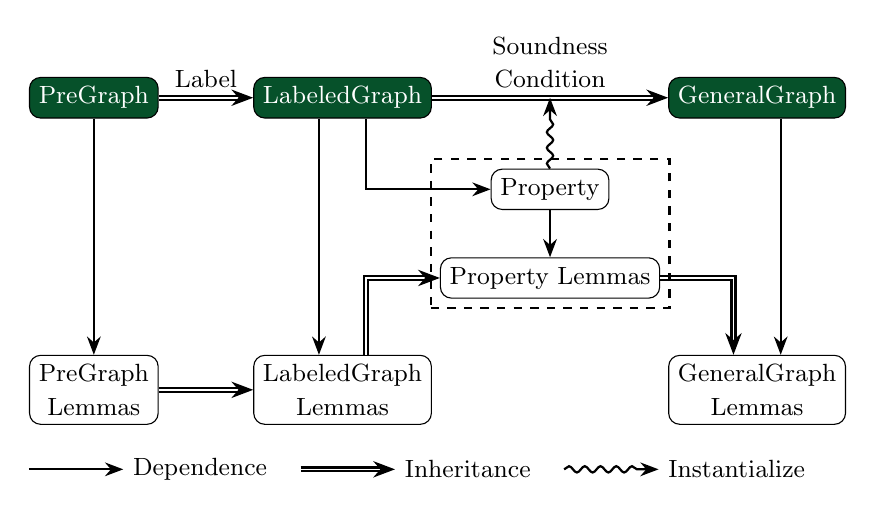
\begin{tikzpicture}
[->/.style={thick,arrows={-Stealth}},
-->/.style={thick,arrows={-Stealth}, decorate, decoration={snake, amplitude=.4mm,segment length=2mm,post length=2mm}},
   realG/.style={shape=rectangle, rounded corners=4pt, draw, fill=darkg},
   propG/.style={shape=rectangle, rounded corners=4pt, draw},
   x=1.5cm, y=1.5cm]
\node[realG] (PG) at (0, 0) {\small\color{white} PreGraph};
\node[realG] (LG) [right=0.8 of PG] {\small\color{white} LabeledGraph};
\node[realG] (GG) [right=2 of LG] {\small\color{white} GeneralGraph};
\draw [double, ->] (PG) -- (LG) node [pos=0.5, above] {\small Label} ;
\draw [double, ->] (LG) -- (GG) node (SC) [pos=0.5, above, align=center]
{\small Soundness \\ \small Condition};
\node[propG] (Prop) [below=0.6 of SC] {\small Property};
\node[propG] (PropL) [below=0.4 of Prop] {\small Property Lemmas};
\node[propG] (PGL) [below=2 of PG, align=center] {\small PreGraph \\\small Lemmas};
\node[propG] (LGL) [below=2 of LG, align=center] {\small LabeledGraph \\\small Lemmas};
\node[propG] (GGL) [below=2 of GG, align=center] {\small GeneralGraph \\\small Lemmas};
\draw [double, ->] (PGL) to (LGL);
%% \draw [double, ->] (LGL) to (GGL);
\draw [->] (PG) to (PGL);
\draw [->] (Prop) to (PropL);
\draw [-->] (Prop) to (SC);
\coordinate [left=0.2 of LG.south] (LGs1);
\coordinate [left=0.2 of LGL.north] (LGLn1);
\draw [->] (LGs1) to (LGLn1);
\coordinate [right=0.2 of LG.south] (LGs2);
\coordinate [right=0.2 of LGL.north] (LGLn2);
\draw [->] (LGs2) |- (Prop);
\draw [double, ->] (LGLn2) |- (PropL);
\coordinate [right=0.2 of GG.south] (GGs);
\coordinate [left=0.2 of GGL.north] (GGLn1);
\coordinate [right=0.2 of GGL.north] (GGLn2);
\draw [double, ->] (PropL) -| (GGLn1);
\draw [->] (GGs) to (GGLn2);
\node [draw, thick, rectangle, dashed, fit=(Prop) (PropL)] {};
\node (legend1) [below right=0.2 and -0.3 of PGL] {\small Dependence};
\coordinate[left=0.8 of legend1]  (l1);
\draw [->] (l1) to (legend1);
\node (legend2) [right=1 of legend1] {\small Inheritance};
\coordinate[left=0.8 of legend2]  (l2);
\draw [double, ->] (l2) to (legend2);
\node (legend3) [right=1 of legend2] {\small Instantialize};
\coordinate[left=0.8 of legend3]  (l3);
\draw [-->] (l3) to (legend3);
\end{tikzpicture}
}
\end{frame}

\section{The Spatial Inference of Graph}
\subsection{Spatial Representation of Graphs}
\begin{frame}[fragile]{Spatial Representation of Graphs}
    \begin{columns}[c]
    \column{.4\textwidth}
    \centering
    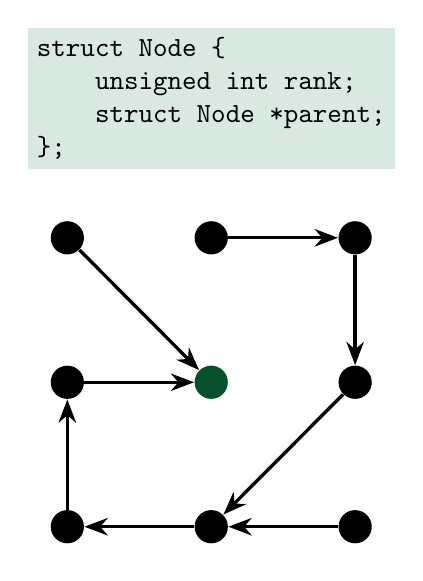
\begin{tikzpicture}[
        gn/.style={circle, inner sep=0pt, minimum size=12pt, fill=black},
        rn/.style={circle, inner sep=0pt, minimum size=12pt, fill=darkg},
        ->/.style={-Stealth, very thick}]
      \node [rectangle, fill=lightg] (struct) {
\begin{BVerbatim}[commandchars=\\\[\]]
\emphd[struct] Node {
    unsigned int rank;
    \emphd[struct] Node *parent;
};
\end{BVerbatim}
      };
      \node[matrix, row sep=40, column sep=40] (graph) [below=15pt of struct] {
        \node[gn] (g1) {}; & \node[gn] (g2) {}; & \node[gn] (g3) {};\\
        \node[gn] (g4) {}; & \node[rn] (g5) {}; & \node[gn] (g6) {};\\
        \node[gn] (g7) {}; & \node[gn] (g8) {}; & \node[gn] (g9) {}; \\
      };
      \draw [->] (g1) to (g5);
      \draw [->] (g2) to (g3);
      \draw [->] (g3) to (g6);
      \draw [->] (g6) to (g8);
      \draw [->] (g9) to (g8);
      \draw [->] (g8) to (g7);
      \draw [->] (g7) to (g4);
      \draw [->] (g4) to (g5);
    \end{tikzpicture}
    \column{.6\textwidth}
    \begin{center}\uncover<2->{
      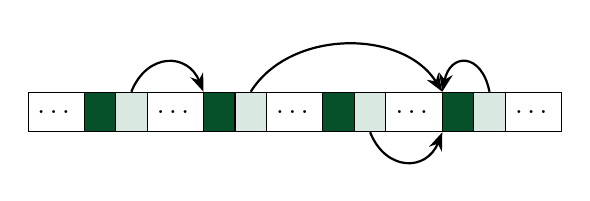
\begin{tikzpicture}[->/.style={-Stealth, thick}]
        \node [rectangle split, rectangle split horizontal, rectangle split parts=13,
          draw, minimum height=0.5cm, rectangle split part fill={white, darkg, lightg,
            white, darkg, lightg, white, darkg, lightg, white, darkg, lightg, white}]
        (heap) {\ldots\nodepart{four}\ldots\nodepart{seven}\ldots\nodepart{ten}\ldots
          \nodepart{thirteen}\ldots};
        \draw[->] (heap.three north)..controls +(0.2, 0.5) and +(-0.2, 0.5)..
        (heap.four split north);
        \draw[->] (heap.six north)..controls +(0.5, 0.8) and +(-0.5, 0.8)..
        (heap.ten split north);
        \draw[->] (heap.nine south)..controls +(0.2, -0.5) and +(-0.2, -0.5)..
        (heap.ten split south);
        \draw[->] (heap.twelve north)..controls +(-0.1, 0.5) and +(0.1, 0.5)..
        (heap.ten split north);
      \end{tikzpicture}}
    \end{center}
  \begin{gather*}
    \uncover<3->{\mathtt{graph\_rep}(\gamma)\,\defeq\,
      \underset{\mathtt{vvalid}(\gamma, v)}{\bigstar}\mathtt{v\_rep}(\gamma, v)\\}
    \uncover<4->{\underset{\{v_1, v_2, \dots, v_n\}}{\bigstar} P \,\defeq \,P(v_1)
      \scon P(v_2)\scon \dots\scon P(v_n)\\}
    \uncover<5->{\mathtt{v\_rep}(\gamma, v)\,\defeq\, v \mapsto
      \mathtt{vlabel}(\gamma, v) \scon \null\\
      (v + 4) \mapsto \mathtt{prt}(\gamma, v)\\}
    \uncover<6->{\mathtt{prt}(\gamma, v)\,\defeq\,
      \begin{cases}
        \mathtt{dst}(\gamma, \mathtt{out}(v)) & \neq\mathtt{null}\\
        v & \text{otherwise}\\
      \end{cases}}
  \end{gather*}
    \end{columns}
\end{frame}

\subsection{Localize Rule}
\begin{frame}{\textsc{Ramify} Rule}
  \credit{\footnotesize (Hobor and Villard)}
  \begin{center}
    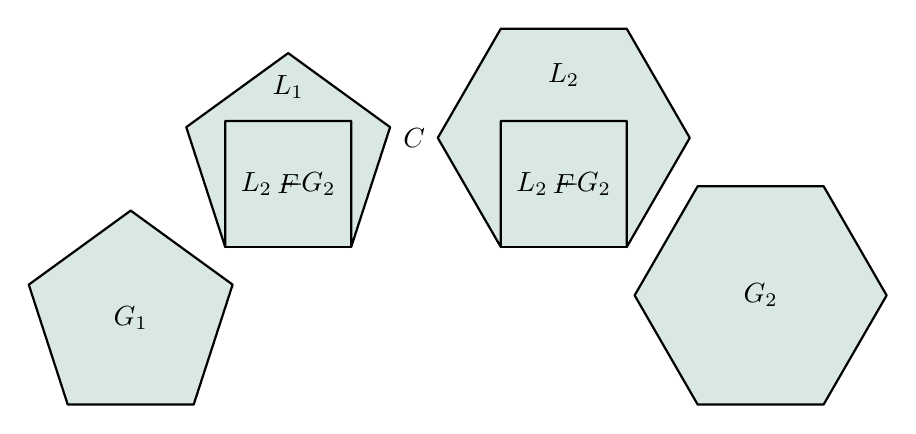
\begin{tikzpicture}[x=1.6cm, y=1.6cm, line join=round]
      \coordinate (six1) at (1, 0);
      \coordinate (six2) at (0.5, 0.866025);
      \coordinate (six3) at (-0.5, 0.866025);
      \coordinate (six4) at (-1, 0);
      \coordinate (six5) at (-0.5, -0.866025);
      \coordinate (six6) at (0.5, -0.866025);
      \coordinate (four1) at (0.5, 0.133975);
      \coordinate (four2) at (-0.5, 0.133975);
      \coordinate (five1) at (0.809017, 0.0850311);
      \coordinate (five2) at (0, 0.672816);
      \coordinate (five3) at (-0.809017, 0.0850311);
      \coordinate (mean four) at (0, -0.366025);
      \coordinate (mean five) at (0, -0.177834);
      \coordinate (mean six) at (0, 0);
      \coordinate (P) at (0, 0.403395);
      \coordinate (Q) at (0, 0.5);
      \draw[thick, fill=lightg] (five1) -- (five2) -- (five3) --
        (six5) -- (six6) -- cycle;
      \node at (mean five) {$G_1$};
      \draw[thick, fill=lightg] ([xshift=8cm]six1) -- ([xshift=8cm]six2) --
      ([xshift=8cm]six3) -- ([xshift=8cm]six4) -- ([xshift=8cm]six5) --
      ([xshift=8cm]six6) -- cycle;
      \node at ([xshift=8cm]mean six) {$G_2$};
      \uncover<3->{\draw[thick, fill=lightg] ([xshift=2cm,yshift=2cm]four1) --
        ([xshift=2cm,yshift=2cm]four2) -- ([xshift=2cm,yshift=2cm]six5) --
        ([xshift=2cm,yshift=2cm]six6) -- cycle;}
      \uncover<2->{\draw[thick, fill=lightg] ([xshift=2cm,yshift=2cm]six6) --
        ([xshift=2cm,yshift=2cm]five1) -- ([xshift=2cm,yshift=2cm]five2) --
        ([xshift=2cm,yshift=2cm]five3) -- ([xshift=2cm,yshift=2cm]six5) --
        ([xshift=2cm,yshift=2cm]four2) -- ([xshift=2cm,yshift=2cm]four1) -- cycle;
        \node at ([xshift=2cm,yshift=2cm]P) {$L_1$};}
      \uncover<3->{\draw[thick, fill=lightg] ([xshift=5.5cm,yshift=2cm]four1) --
        ([xshift=5.5cm,yshift=2cm]four2) -- ([xshift=5.5cm,yshift=2cm]six5) --
        ([xshift=5.5cm,yshift=2cm]six6) -- cycle;}
      \uncover<2->{\draw[thick, fill=lightg] ([xshift=5.5cm,yshift=2cm]six6) --
        ([xshift=5.5cm,yshift=2cm]six1) -- ([xshift=5.5cm,yshift=2cm]six2) --
        ([xshift=5.5cm,yshift=2cm]six3) -- ([xshift=5.5cm,yshift=2cm]six4) --
        ([xshift=5.5cm,yshift=2cm]six5) -- ([xshift=5.5cm,yshift=2cm]four2) --
        ([xshift=5.5cm,yshift=2cm]four1) -- cycle;
        \node at ([xshift=5.5cm,yshift=2cm]Q) {$L_2$};}
      \node<3,4> at ([xshift=2cm,yshift=2cm]mean four) {$F$};
      \node<3,4> at ([xshift=5.5cm,yshift=2cm]mean four) {$F$};
      \node<5-> at ([xshift=2cm,yshift=2cm]mean four) {$L_2 \wand G_2$};
      \node<5-> at ([xshift=5.5cm,yshift=2cm]mean four) {$L_2 \wand G_2$};
      \node at ([xshift=3.6cm, yshift=2cm]mean six) {$C$};
    \end{tikzpicture}
  \end{center}
  \begin{gather*}
    \frac{\uncover<2->{\{L_1\}\,C\,\{L_2\}}\quad
      \uncover<6->{G_1 \vdash L_1 \scon (L_2 \wand G_2)}}
         {\{G_1\}\,C\,\{G_2\}}\;
         \uncover<6->{(\mathtt{mod}(C)\cap\mathtt{fv}(L_2 \wand G_2)=\emptyset)\\}
         \uncover<4,5>{\alert{\text{Hint: }\forall P, Q\,.\, P \scon (P \wand Q)
             \vdash Q}}
  \end{gather*}
\end{frame}

\begin{frame}{Our \textsc{Localize} Rule}
  \begin{equation*}
    \frac{\{ L_1 \}\,C\,\{{\color{red}{\exists x \,.\,}} L_2\} \qquad
      G_1 \vdash L_1 \scon R \qquad
      R \vdash
      {\color{red}{\forall x \,.\,(}}
      L_2 \wand G_2{\color{red}{)}}}
         {\{ G_1 \} \,C\, \{{\color{red}{\exists x \,.\,}} G_2 \}} ~~(\dagger)
  \end{equation*}
  \vspace{0.5em}
  \begin{align*}
   (\dagger)~~\mathtt{mod}(C)\cap\mathtt{fv}(R)=\emptyset\\
  \end{align*}
  \vfill
Comparing to Hobor and Villard's Ramify rule:
  \begin{gather*}
    \frac{{\{L_1\}\,C\,\{L_2\}}\quad
      {G_1 \vdash L_1 \scon (L_2 \wand G_2)}}
         {\{G_1\}\,C\,\{G_2\}}\; ~~ (\ddagger)
  \end{gather*}
  \begin{align*}
  (\ddagger) ~~ \mathtt{mod}(C)\cap\mathtt{fv}(L_2 \wand G_2)=\emptyset
  \end{align*}
\end{frame}

\section{Verification of the Find function}

\subsection{Specification}
\begin{frame}{The Specification of Find}
  \centering
  \colorbox{lightg}{\parbox{.9\textwidth}{
      \begin{description}
      \item[{\bf PRE:}] $\mathtt{graph\_rep}(\gamma) \wedge \mathtt{vvalid}(\gamma, x)$
      \item[{\bf POST:}] $\exists \gamma', \mathit{ret}\;\text{.}\;\mathtt{graph\_rep}(\gamma')\wedge\mathtt{uf\_eq}(\gamma, \gamma') \wedge \mathtt{root}(\gamma', x, \mathit{ret})$
  \end{description}}}
  \pause
  \vskip10pt
  \colorbox{lightg}{\parbox{.9\textwidth}{
      \begin{align*}
        \mathtt{graph\_rep}(\gamma)\;\defeq\; &
        \underset{\mathtt{vvalid}(\gamma, v)}{\bigstar}\mathtt{v\_rep}(\gamma, v)\\
        \mathtt{root}(\gamma, x, \mathit{ret}) \;\defeq\; &\gamma \vDash x \leadsto \mathit{ret} \wedge
        \forall y.~ \gamma \vDash \mathit{ret} \leadsto y \Rightarrow y = \mathit{ret}\\
        \mathtt{uf\_eq}(\gamma_1, \gamma_2)\; \defeq\; &\big(\forall x.~
        \mathtt{vvalid}(\gamma_1, x)\Leftrightarrow \mathtt{vvalid}(\gamma_2,x)\big)
        \, \wedge\, \null\\
        & \forall x, r_1, r_2.~ \mathtt{root}(\gamma_1, x, r_1) \Rightarrow\\
        &\mathtt{root}(\gamma_2, x, r_2) \Rightarrow r_1 = r_2
      \end{align*}
    }}
\end{frame}

\subsection{Proof Skeleton}

\begin{frame}{Proof Skeleton of Find}
  \centering
  \begin{tikzpicture}[node distance=0.4mm]
    \node (line 0) {\color<3-10>{lightgray}{$\{\mathtt{graph\_rep}(\gamma) \wedge
      \mathtt{vvalid}(\gamma, \mathtt{x})\}$}};
    \node (line 1) [below = of line 0] {\color<3-10>{lightgray}
      {\Verb|p = x -> parent;|}};
    \onslide<2->{\node (line 2) [below = of line 1]
      {\color<5-10>{lightgray}{$\{\mathtt{graph\_rep}(\gamma) \wedge
      \mathtt{vvalid}(\gamma, \mathtt{x})\wedge
      \mathtt{p}=\mathtt{prt}(\gamma, \mathtt{x})\}$}};}
    \node (line 3) [below = of line 2] {\color<2,5-10>{lightgray}
      {\Verb|p0 = find(p);|}};
    \onslide<4->{\node (line 4) [below = of line 3] {\color<7,9,10>{lightgray}
        {$\{\mathtt{graph\_rep}
          (\gamma_1)\wedge\mathtt{uf\_eq}(\gamma, \gamma_1) \wedge
          \mathtt{root}(\gamma_1, \mathtt{p}, \mathtt{p0})\wedge
          \mathtt{p}=\mathtt{prt}(\gamma, \mathtt{x})\}$}};}
    \onslide<7->{\node (line 5) [below = of line 4] {\color<9,10>{lightgray}
        {$\uncover<8->{\alert{\searrow}} \{\mathtt{x}\mapsto
          \mathtt{vlabel}(\gamma_1, \mathtt{x}),
          \mathtt{prt}(\gamma_1, \mathtt{x})\}$}};}
      \node (line 6) [below = of line 5] {\color<2-4,9,10>{lightgray}
        {\Verb|x -> parent = p0|}};
      \onslide<7->{\node (line 7) [below = of line 6] {\color<9,10>{lightgray}
          {$\uncover<8->{\alert{\swarrow}}
          \{\mathtt{x}\mapsto \mathtt{vlabel}(\gamma_1, \mathtt{x}), \mathtt{p0}\}$}};}
      \onslide<6->{\node (line 8) [below = of line 7] {\color<7>{lightgray}
          {$\{\mathtt{graph\_rep}
          (\gamma_2)\wedge\gamma_2=\mathtt{redirect\_parent}(\gamma_1,\mathtt{x},
          \mathtt{p0}) \wedge\dots\}$}};}
      \onslide<10->{\node (line 9) [below = of line 8] {$\{\mathtt{graph\_rep}
          (\gamma_2)\wedge\mathtt{uf\_eq}(\gamma, \gamma_2) \wedge \mathtt{root}
          (\gamma_2, \mathtt{x}, \mathtt{p0})\}$};}
      \onslide<1-11>{\node (line 10) [below = of line 9]
        {\color<2,5-8>{lightgray}{$\{\exists \gamma'.~
         \mathtt{graph\_rep}(\gamma')\wedge\mathtt{uf\_eq}(\gamma,
            \gamma') \wedge \mathtt{root}(\gamma', \mathtt{x}, \mathtt{p0})\}$}};}
  \end{tikzpicture}
\end{frame}

\begin{frame}{Proof Obligation of Find}
  \centering
  \colorbox{lightg}{\parbox{.9\textwidth}{
  \begin{align*}
    \mathtt{graph\_rep}(\gamma_1) \vdash & \big(\mathtt{x}\mapsto
    \mathtt{vlabel}(\gamma_1, \mathtt{x}), \mathtt{prt}(\gamma_1, \mathtt{x})\big)
    \scon \null\\
    & \Big(\big(\mathtt{x}\mapsto \mathtt{vlabel}(\gamma_1, \mathtt{x}),
    \mathtt{p0}\big) \wand \null\\
    & \mathtt{graph\_rep}\big(\mathtt{redirect\_parent}(\gamma_1,\mathtt{x},
    \mathtt{p0})\big)\Big)
  \end{align*}}}
  \pause
  \vskip15pt
  \colorbox{lightg}{\parbox{.9\textwidth}{
  \begin{align*}
    & \mathtt{uf\_eq}(\gamma, \gamma_1) \Rightarrow \mathtt{root}(\gamma_1, \mathtt{p},
    \mathtt{p0}) \Rightarrow \mathtt{dst}\big(\gamma, \mathtt{out}(\mathtt{x})\big)=
    \mathtt{p}\\
    & \gamma_2=\mathtt{redirect\_parent}(\gamma_1,\mathtt{x},\mathtt{p0}) \Rightarrow\\
    & \mathtt{uf\_eq}(\gamma, \gamma_2) \wedge \mathtt{root}(\gamma_2, \mathtt{x},
    \mathtt{p0})
  \end{align*}}}
\end{frame}

\section{A Garbage Collector}

\begin{frame}{A Generational Garbage Collector}
  \begin{itemize}
  \item 12 generations; mutator allocates only into the first
  \item Functional mutator, so no backward pointers
  \pause
  \item Cheney's mark-and-copy collects generation to its successor
  \item Receiving generation may exceed fullness bound, \\
  triggering cascade of further pairwise collections
  \pause
  \item Most tasks are handled by two key functions: \texttt{forward} (to copy
  individual objects) and \texttt{do\_scan} (to repair the copied objects)
  \end{itemize}
\end{frame}

\begin{frame}{Separation between pure and spatial reasoning}
  \centering
  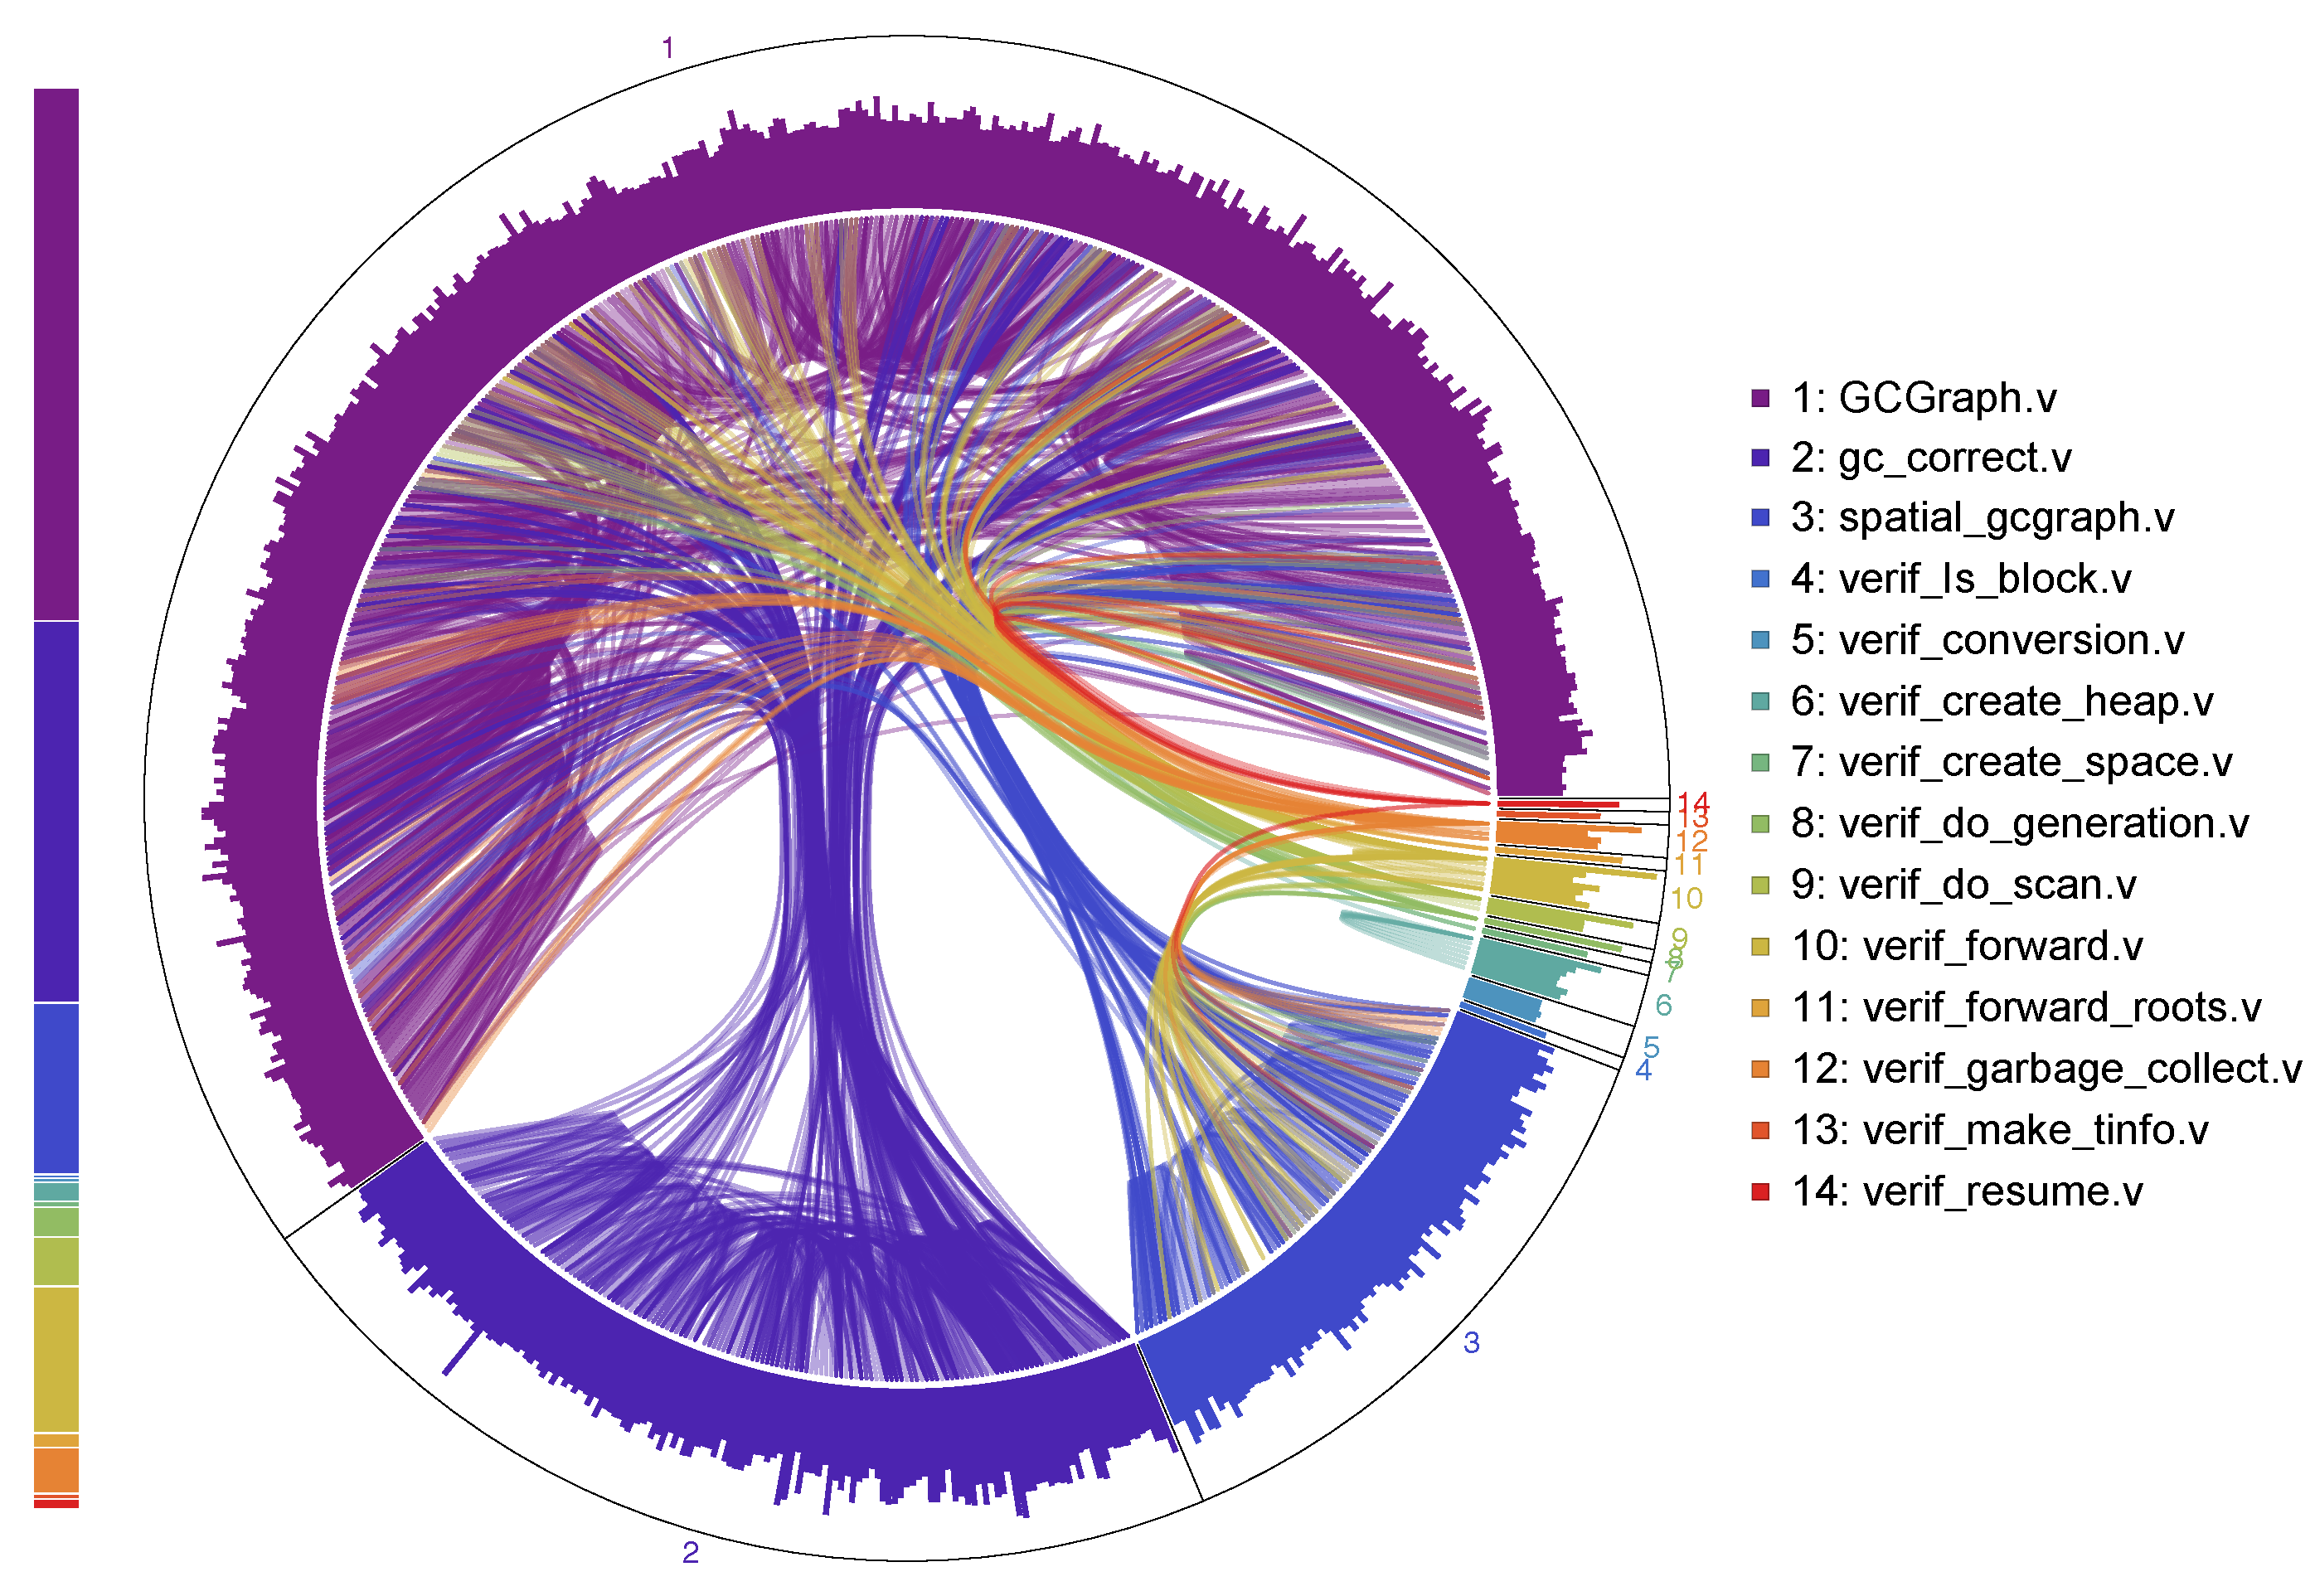
\includegraphics[width=0.9\textwidth]{certigc_theorems.pdf}
\end{frame}

\begin{frame}[fragile]{Undefined behavior in C}

  \begin{itemize}
  \item Double-bounded pointer comparisons:
    \begin{Verbatim}
int Is_from(value * from_start,
            value * from_limit, value * v) {
    return (from_start <= v && v < from_limit); }
    \end{Verbatim}
    Resolved using CompCert's ``extcall\_properties''.
    \pause
  \item A classic OCaml trick:
    \begin{Verbatim}
int test_int_or_ptr (value x) {
    return (int)(((intnat)x)&1); }
    \end{Verbatim}
    Discussing \texttt{char} alignment issues with CompCert.
  \end{itemize}
\end{frame}

\end{document}
